\documentclass[9pt]{beamer}
\mode<presentation>

% Theme choice:
\usetheme{Madrid}%Darmstadt 

\definecolor{univBlue}{RGB}{0, 57, 145}
\definecolor{univLightBlue}{RGB}{71, 115, 169}
\definecolor{univSoftBlue}{RGB}{147, 172, 203}

\usecolortheme[RGB={0, 57, 145}]{structure}
 \usefonttheme{structurebold} 
\setbeamercovered{invisible}
%\setbeamertemplate{navigation symbols}{}
\usepackage{dynblocks}
\usepackage{textpos}
\usepackage{amsfonts}
\usepackage{amsmath}
\usepackage{amssymb}
\usepackage{amsthm}
\usepackage{subcaption}
\usepackage{tikz}
\usetikzlibrary{shapes.geometric, shapes.symbols, arrows.meta, positioning, shapes.multipart}
\newtheorem{teorema}{Teorema}\usepackage{mathtools}
\renewcommand{\proofname}{Prova}
\usepackage[portuguese]{babel}
\usepackage{pifont}
\uselanguage{Portuguese}
\languagepath{Portuguese}

\deftranslation[to=Portuguese]{Theorem}{Teorema}
\deftranslation[to=Portuguese]{Lemma}{Lema}
\deftranslation[to=Portuguese]{Corollary}{Corolário}
\deftranslation[to=Portuguese]{Proof}{Prova}

\usepackage{dutchcal}
\usepackage{hyperref}
\usepackage[utf8]{inputenc}
\usepackage[T1]{fontenc}
\usepackage{amsthm}


\usepackage[affil-it]{authblk} 
\usepackage{etoolbox}
\usepackage{lmodern}
\usepackage{listings}
\usepackage{xcolor}

\definecolor{codegreen}{rgb}{0,0.6,0}
\definecolor{codegray}{rgb}{0.5,0.5,0.5}
\definecolor{codepurple}{rgb}{0.58,0,0.82}
\definecolor{backcolour}{rgb}{0.95,0.95,0.92}

\lstset{
    language=Java,
    backgroundcolor=\color{backcolour},   
    commentstyle=\color{codegreen},
    keywordstyle=\color{univBlue},
    numberstyle=\tiny\color{codegray},
    stringstyle=\color{codepurple},
    basicstyle={\ttfamily\small},
    breakatwhitespace=false,         
    breaklines=true,                 
    captionpos=b,                    
    keepspaces=true,                 
    numbers=left,                    
    numbersep=5pt,                  
    showspaces=false,                
    showstringspaces=false,
    showtabs=false,                  
    tabsize=2
}

\makeatletter
\patchcmd{\@maketitle}{\LARGE \@title}{\fontsize{18}{19.2}\selectfont\@title}{}{}
\makeatother

\renewcommand\Authfont{\fontsize{12}{14.4}\selectfont}
\renewcommand\Affilfont{\fontsize{9}{10.8}\itshape}

% Title page details: 
\title[Presentation]{Programação Orientada a Objetos} %add title


\institute[UniRV]{\textbf{\large  \textcolor{univBlue}{\textbf{\large
Herança e Composição em Java
}} %add name 
% \hspace{0.5pt}
\\ \qquad
\\Professor: Me. Sergio Souza Novak 
\\Faculdade de Engenharia de Software}
} 
% \titlegraphic{\includegraphics[width=5cm]{msu.eps}}
\titlegraphic{
\includegraphics[width=3cm]{universidade_logo_novo.png}}
\date{}

% Logo only on title page
%\logo{
\includegraphics[width=1cm,keepaspectratio]{Logo.png}}
\usepackage[pscoord]{eso-pic}


\begin{document}

% Title page frame
%\begin{frame}
    %\titlepage 
%\end{frame}
\frame[plain]{\titlepage}
%logo
\AddToShipoutPictureFG{
    \put(\LenToUnit{.92\paperwidth},
    \LenToUnit{.185\paperheight})
    {\vtop{{\null}
    \makebox{
\includegraphics[width=.8cm,keepaspectratio]{universidade_logo_novo.png}}}}}


\begin{frame}{Sumário}
  \tableofcontents
\end{frame}

\section{Introdução}

% \begin{frame}{Introdução ao Polimorfismo}

% \centering

% \begin{tikzpicture}

% % Caixa principal
% \node[draw=blue!60, fill=blue!10, rounded corners=10pt, 
%       minimum width=10cm, minimum height=4cm] (box) {};

% % Título dentro da caixa
% \node[above=0.3cm of box.north, font=\large\bfseries, text=blue!80] 
% {O que é Polimorfismo?};

% % Texto interno
% \node[align=center] at (box.center) {
%     \textbf{\textcolor{blue!70}{Poli}} = muitos \\
%     \vspace{0.3cm}
%     \textbf{\textcolor{blue!70}{Morfismo}} = formas \\
%     \vspace{0.5cm}
%     \textbf{\Large Polimorfismo = Muitas Formas}
% };

% % Ícones representando "formas"
% \node[draw, circle, fill=red!20, minimum size=0.8cm] at (-3,-2.2) {};
% \node[draw, rectangle, fill=green!20, minimum width=1cm, minimum height=0.8cm] at (-1.5,-2.2) {};
% \node[draw, diamond, fill=yellow!30, minimum size=0.9cm] at (0,-2.2) {};
% \node[draw, star, star points=5, fill=purple!30, minimum size=0.9cm] at (1.5,-2.2) {};

% % Legenda
% \node at (0,-3.2) {\small Diferentes formas, mesmo conceito};

% \end{tikzpicture}

% \end{frame}

\section{Conceitos de Herança}
\begin{frame}{O que é Herança?}
    \begin{itemize}
        \item \textbf{Conceito:} É um mecanismo que permite que uma classe (subclasse) herde atributos e métodos de outra classe (superclasse).
        \item \textbf{Reutilização:} Promove a reutilização de código, evitando duplicações.
        \item \textbf{Relação "É um":} Define uma relação onde a subclasse é uma especialização da superclasse.
        \item \textbf{Exemplo:} Um \textit{Cachorro} \textbf{é um} \textit{Animal}.
    \end{itemize}
    
    \centering
    \begin{tikzpicture}[node distance=2cm]
        \node[draw=univBlue, fill=univSoftBlue, rounded corners, minimum width=3cm, text=white] (super) {Superclasse (Pai)};
        \node[draw=univBlue, fill=univLightBlue, rounded corners, minimum width=3cm, below=of super, text=white] (sub) {Subclasse (Filho)};
        \draw[->, thick, univBlue, >=stealth] (sub) -- (super) node[midway, right, text=univBlue] {herda de};
    \end{tikzpicture}
\end{frame}

\begin{frame}{Como a Herança ocorre?}
    \begin{itemize}
        \item Em Java, utilizamos a palavra-chave \texttt{extends}.
        \item Uma classe só pode estender \textbf{uma única} classe (Herança Simples).
        \item A subclasse ganha acesso a todos os membros \texttt{public} e \texttt{protected} da superclasse.
    \end{itemize}
    
    \begin{block}{Sintaxe}
        \texttt{public class Subclasse \textbf{extends} Superclasse \{ ... \}}
    \end{block}
\end{frame}

\section{Exemplo: Hierarquia Animal}
\begin{frame}{UML: Hierarquia Animal}
    \centering
    \begin{tikzpicture}[
        umlclass/.style={
            draw=univBlue, 
            rectangle split, 
            rectangle split parts=3, 
            fill=univSoftBlue, 
            minimum width=3cm, 
            font=\small\ttfamily,
            align=left,
            text=white
        },
        inheritance/.style={
            -{Triangle[open]}, 
            thick,
            univBlue
        },
        node distance=2cm and 1cm
    ]

    % Superclasse
    \node[umlclass, fill=univLightBlue] (animal) {
        \textbf{Animal}
        \nodepart{second}
        nome: String
        \nodepart{third}
        comer(): void
    };

    % Subclasses
    \node[umlclass, below left=of animal] (cachorro) {
        \textbf{Cachorro}
        \nodepart{second}
        \nodepart{third}
        latir(): void
    };
    
    \node[umlclass, below right=of animal] (gato) {
        \textbf{Gato}
        \nodepart{second}
        \nodepart{third}
        miar(): void
    };

    % Setas
    \draw[inheritance] (cachorro.north) -- ++(0,0.5) -| (animal.south);
    \draw[inheritance] (gato.north) -- ++(0,0.5) -| (animal.south);

    \end{tikzpicture}
\end{frame}

\begin{frame}[fragile]{Exemplo de Herança: Superclasse}
\begin{lstlisting}
// Classe Base (Superclasse)
public class Animal {
    String nome;

    public void comer() {
        System.out.println(nome + " esta comendo...");
    }
}
\end{lstlisting}
\end{frame}

\begin{frame}[fragile]{Exemplo de Herança: Subclasse Cachorro}
\begin{lstlisting}
// Subclasse
public class Cachorro extends Animal {
    public void latir() {
        System.out.println(nome + " diz: Au Au!");
    }
}
\end{lstlisting}
\end{frame}

\begin{frame}[fragile]{Exemplo de Herança: Subclasse Gato}
\begin{lstlisting}
// Subclasse
public class Gato extends Animal {
    public void miar() {
        System.out.println(nome + " diz: Miau!");
    }
}
\end{lstlisting}
\end{frame}

\begin{frame}[fragile]{Exemplo de Herança: Uso}
\begin{lstlisting}
public class Main {
    public static void main(String[] args) {
        Cachorro c1 = new Cachorro();
        c1.nome = "Rex";
        c1.comer(); // Herdado de Animal
        c1.latir(); // Proprio de Cachorro

        Gato g1 = new Gato();
        g1.nome = "Luna";
        g1.comer(); // Herdado de Animal
        g1.miar();  // Proprio de Gato
    }
}
\end{lstlisting}
\end{frame}
\begin{frame}{Superclasse e Subclasses}

\begin{block}{Superclasse}
\textbf{Classe Animal}
\begin{itemize}
    \item Define características comuns:
    \begin{itemize}
        \item Atributo: \texttt{nome}
        \item Método: \texttt{comer()}
    \end{itemize}
    \item Serve como base para outras classes
\end{itemize}
\end{block}

\begin{exampleblock}{Subclasses}
\textbf{Cachorro e Gato}
\begin{itemize}
    \item Herdam de \texttt{Animal} usando \texttt{extends}
    \item Reutilizam:
    \begin{itemize}
        \item \texttt{nome}
        \item \texttt{comer()}
    \end{itemize}
    \item \textbf{Especialização:}
    \begin{itemize}
        \item Cachorro → \texttt{latir()}
        \item Gato → \texttt{miar()}
    \end{itemize}
\end{itemize}
\end{exampleblock}

\end{frame}

\section{Exemplo Prático: Equipamentos Médicos}
\begin{frame}{Equipamento de Raio-X (Base)}
    \begin{columns}
        \begin{column}{\textwidth}
            \begin{itemize}
                \item \textbf{Conceito:} Base tecnológica para diagnósticos por imagem via radiação.
                \item \textbf{Funcionamento:} Produção de feixes de elétrons em uma ampola de vácuo.
                \item \textbf{Atributos Comuns:} 
                \begin{itemize}
                    \item Modelo e Fabricante
                    \item Tensão de Operação (kV)
                \end{itemize}
            \end{itemize}
        \end{column}
    \end{columns}
\end{frame}

\begin{frame}{Tomógrafo Computadorizado}
    \begin{columns}
        \begin{column}{0.6\textwidth}
            \begin{itemize}
                \item \textbf{Especialização:} Realiza múltiplos cortes (slices) do corpo.
                \item \textbf{Funcionalidade:} Reconstrução de imagens em 3D.
                \item \textbf{Uso:} Diagnóstico detalhado de órgãos internos e vasos.
            \end{itemize}
        \end{column}
        \begin{column}{0.4\textwidth}
            \centering
            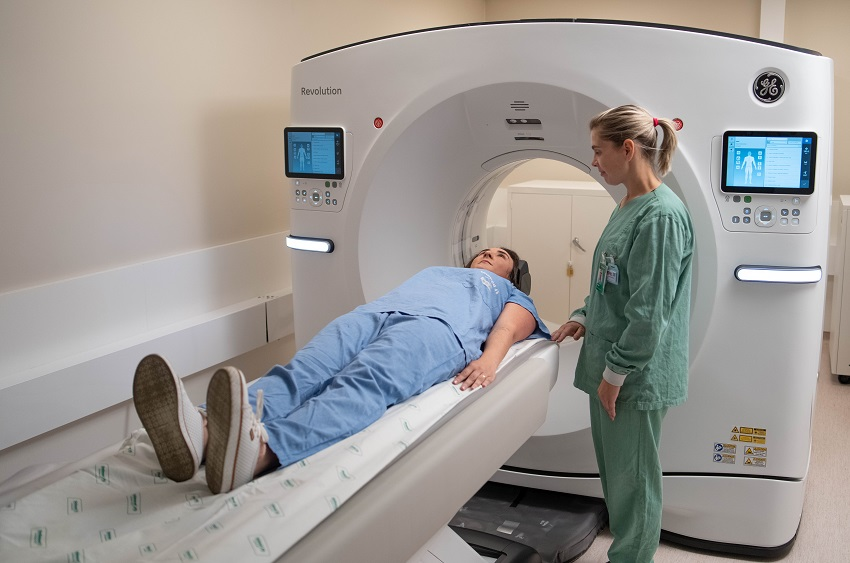
\includegraphics[width=\textwidth]{tomografo.jpg}
        \end{column}
    \end{columns}
\end{frame}

\begin{frame}{Mamógrafo}
    \begin{columns}
        \begin{column}{0.6\textwidth}
            \begin{itemize}
                \item \textbf{Especialização:} Exames de tecidos mamários.
                \item \textbf{Funcionalidade:} Compressão mecânica para melhor nitidez.
                \item \textbf{Uso:} Prevenção e diagnóstico de câncer de mama.
            \end{itemize}
        \end{column}
        \begin{column}{0.4\textwidth}
            \centering
            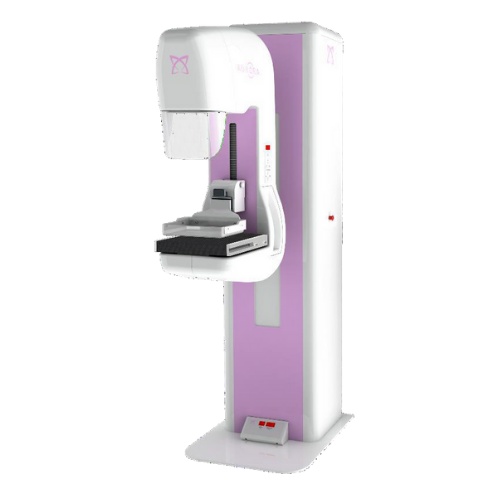
\includegraphics[width=\textwidth]{mamografo.png}
        \end{column}
    \end{columns}
\end{frame}

\begin{frame}{Densitômetro Ósseo}
    \begin{columns}
        \begin{column}{0.6\textwidth}
            \begin{itemize}
                \item \textbf{Especialização:} Medição da densidade mineral óssea.
                \item \textbf{Funcionalidade:} Cálculo do T-Score.
                \item \textbf{Uso:} Diagnóstico de Osteoporose e Osteopenia.
            \end{itemize}
        \end{column}
        \begin{column}{0.4\textwidth}
            \centering
            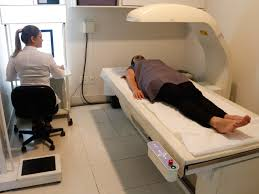
\includegraphics[width=0.9\textwidth]{densitometro.jpeg}
        \end{column}
    \end{columns}
\end{frame}

\begin{frame}{UML: Equipamentos Médicos}
    \centering
    \begin{tikzpicture}[
        umlclass/.style={
            draw=univBlue, 
            rectangle split, 
            rectangle split parts=3, 
            fill=univSoftBlue, 
            minimum width=3.5cm, 
            font=\scriptsize\ttfamily,
            align=left,
            text=white
        },
        inheritance/.style={
            -{Triangle[open]}, 
            thick,
            univBlue
        },
        node distance=1.8cm and 0.5cm
    ]

    % Superclasse
    \node[umlclass, fill=univLightBlue] (raiox) {
        \textbf{EquipamentoRaioX}
        \nodepart{second}
        \# modelo: String\\
        \# fabricante: String\\
        \# kvMaximo: double
        \nodepart{third}
        + ligar(): void\\
        + emitirRadiacao(): void
    };

    % Subclasses
    \node[umlclass, below=of raiox] (mamografo) {
        \textbf{Mamografo}
        \nodepart{second}
        - pressao: double
        \nodepart{third}
        + comprimir(): void
    };

    \node[umlclass, left=of mamografo] (tomografia) {
        \textbf{Tomografia}
        \nodepart{second}
        - numCortes: int
        \nodepart{third}
        + reconstruir3D(): void
    };

    \node[umlclass, right=of mamografo] (densitometro) {
        \textbf{Densitometro}
        \nodepart{second}
        \nodepart{third}
        + calcularTScore(): void
    };

    % Setas
    \draw[inheritance] (tomografia.north) -- ++(0,0.5) -| (raiox.south);
    \draw[inheritance] (mamografo.north) -- (raiox.south);
    \draw[inheritance] (densitometro.north) -- ++(0,0.5) -| (raiox.south);

    \end{tikzpicture}
\end{frame}

\begin{frame}[fragile]{Exemplo Complexo: Superclasse}
\begin{lstlisting}
public class EquipamentoRaioX {
    protected String modelo;
    protected String fabricante;
    protected double kvMaximo; // Kilo-voltagem

    public void ligar() {
        System.out.println("Equipamento " + modelo + " ligado.");
    }

    public void emitirRadiacao() {
        System.out.println("Emitindo raios-X em " + kvMaximo + "kV...");
    }
}
\end{lstlisting}
\end{frame}

\begin{frame}[fragile]{Subclasse: Tomografia}
\begin{lstlisting}
public class Tomografia extends EquipamentoRaioX {
    private int numeroCortes;

    public void reconstruir3D() {
        System.out.println("Reconstruindo imagem de " + 
                            numeroCortes + " cortes.");
    }
}
\end{lstlisting}
\end{frame}

\begin{frame}[fragile]{Subclasse: Mamógrafo}
\begin{lstlisting}
public class Mamografo extends EquipamentoRaioX {
    private double pressaoCompressor;

    public void comprimir() {
        System.out.println("Comprimindo com " + 
                            pressaoCompressor + "kgf.");
    }
}
\end{lstlisting}
\end{frame}

\begin{frame}[fragile]{Subclasse: Densitômetro Ósseo}
\begin{lstlisting}
public class Densitometro extends EquipamentoRaioX {
    public void calcularTScore() {
        System.out.println("Calculando densidade ossea...");
    }
}
\end{lstlisting}
\end{frame}

\begin{frame}[fragile]{Exemplo Complexo: Uso}
\begin{lstlisting}
public class TesteClinica {
    public static void main(String[] args) {
        Tomografia t1 = new Tomografia();
        t1.modelo = "Aquilion";
        t1.ligar(); // Herdado
        t1.reconstruir3D(); // Especifico

        Mamografo m1 = new Mamografo();
        m1.modelo = "Senographe";
        m1.emitirRadiacao(); // Herdado
        m1.comprimir(); // Especifico
    }
}
\end{lstlisting}
\end{frame}
\begin{frame}
\centering

\vspace{1cm}

{\Huge \textbf{Herança e Reutilização}}

\vspace{0.8cm}

{\large Como classes compartilham comportamento}

\vspace{1.5cm}

\begin{tikzpicture}
    % Linha decorativa
    \draw[univBlue, thick] (-4,0) -- (4,0);

    % Ícones simples
    \node[draw=univBlue, circle, fill=univLightBlue, minimum size=0.8cm, text=white] at (-2,0.8) {};
    \node[draw=univBlue, rectangle, fill=univSoftBlue, minimum width=1cm, minimum height=0.7cm, text=white] at (0,0.8) {};
    \node[draw=univBlue, diamond, aspect=2, fill=univSoftBlue!50, minimum size=0.8cm, text=white] at (2,0.8) {};
\end{tikzpicture}

\vfill

\end{frame}

\section{Modificadores de Acesso e Herança}
\begin{frame}[fragile]{Modificador \texttt{private} e Herança}
\begin{itemize}
    \item \textbf{Acesso:} Apenas dentro da própria classe.
    \item \textbf{Herança:}
    \begin{itemize}
        \item  Não é acessível diretamente na subclasse
        \item Ainda existe no objeto (é herdado, mas oculto)
    \end{itemize}
    
    \item \textbf{Exemplo:}
\end{itemize}

\begin{lstlisting}
class Animal {
    private String nome;
}

class Cachorro extends Animal {
    void teste() {
        // nome = "Rex"; ERRO
    }
}
\end{lstlisting}

\begin{block}{Conclusão}
Use getters/setters para acessar atributos privados.
\end{block}
\end{frame}
\begin{frame}[fragile]{Modificador \texttt{private} e Herança}
\begin{itemize}
    \item \textbf{Acesso:} Apenas dentro da própria classe.
    \item \textbf{Herança:}
    \begin{itemize}
        \item  Não é acessível diretamente na subclasse
        \item Ainda existe no objeto (é herdado, mas oculto)
    \end{itemize}
    
    \item \textbf{Exemplo:}
\end{itemize}

\begin{lstlisting}
class Animal {
    private String nome;
}

class Cachorro extends Animal {
    void teste() {
        // nome = "Rex";  ERRO
    }
}
\end{lstlisting}

\begin{block}{Conclusão}
Use getters/setters para acessar atributos privados.
\end{block}
\end{frame}
\begin{frame}[fragile]{Modificador \texttt{public} e Herança}
\begin{itemize}
    \item \textbf{Acesso:} Qualquer classe em qualquer lugar.
    
    \item \textbf{Herança:}
    \begin{itemize}
        \item  Totalmente acessível na subclasse
        \item  Pode ser usado livremente
    \end{itemize}

    \item \textbf{Exemplo:}
\end{itemize}

\begin{lstlisting}
class Animal {
    public String nome;
}

class Cachorro extends Animal {
    void teste() {
        nome = "Rex"; //  permitido
    }
}
\end{lstlisting}

\begin{block}{Conclusão}
Fácil acesso, mas expõe demais os dados.
\end{block}
\end{frame}
\begin{frame}[fragile]{Modificador \texttt{default} (package-private)}
\begin{itemize}
    \item \textbf{Sem modificador declarado}
    
    \item \textbf{Acesso:}
    \begin{itemize}
        \item  Apenas dentro do mesmo pacote
    \end{itemize}

    \item \textbf{Herança:}
    \begin{itemize}
        \item Acessível se a subclasse estiver no mesmo pacote
        \item  Não acessível em pacotes diferentes
    \end{itemize}

    \item \textbf{Exemplo:}
\end{itemize}

\begin{lstlisting}
class Animal {
    String nome; // default
}

class Cachorro extends Animal {
    void teste() {
        nome = "Rex"; //  mesmo pacote
    }
}
\end{lstlisting}

\begin{alertblock}{Importante}
Não funciona bem para herança entre pacotes.
\end{alertblock}
\end{frame}


\section{A Palavra-chave \texttt{super}}
\begin{frame}{A Palavra-chave \texttt{super}}

\begin{columns}

% Coluna da explicação
\column{0.55\textwidth}

\begin{block}{O que é?}
Referência direta à \textbf{superclasse} imediata
\end{block}

\begin{block}{Para que serve?}
\begin{itemize}
    \item Chamar o construtor da superclasse
    \item Acessar métodos sobrescritos
    \item Acessar atributos herdados
\end{itemize}
\end{block}

\begin{alertblock}{Regra de Ouro}
\texttt{super()} deve ser a \textbf{primeira instrução} no construtor
\end{alertblock}

% Coluna do diagrama
\column{0.45\textwidth}

\centering

\begin{tikzpicture}[node distance=2cm]

% Superclasse
\node[draw=univBlue, fill=univSoftBlue, rounded corners, minimum width=1cm, minimum height=1cm, text=white] (animal) {Animal};

% Subclasse
\node[draw=univBlue, fill=univLightBlue, rounded corners, below of=animal, text=white] (cachorro) {Cachorro};

% Seta herança
\draw[->, thick, univBlue] (cachorro) -- (animal);

% Texto construtor super
\node[right=1.5cm of cachorro, align=left] (codigo) {
\texttt{Cachorro() \{}\\
\texttt{\ \ super();}\\
\texttt{\}}
};

% Seta indicando chamada
\draw[->, dashed, univBlue] (codigo.west) -- (cachorro.east);

\node[above=0.2cm of animal, text=univBlue] {\small Superclasse};
\node[below=0.2cm of cachorro, text=univBlue] {\small Subclasse};

\end{tikzpicture}

\end{columns}

\end{frame}

\begin{frame}{Chamando Construtores com \texttt{super()}}
    \begin{itemize}
        \item Quando criamos um objeto da subclasse, o Java precisa inicializar a superclasse primeiro.
        \item Se a superclasse não tiver um construtor padrão (vazio), a subclasse \textbf{deve} chamar explicitamente um construtor da superclasse.
    \end{itemize}
    \begin{block}{Sintaxe}
        \texttt{super(parâmetros);}
    \end{block}
\end{frame}

\begin{frame}[fragile]{Exemplo: \texttt{super()} no Construtor}
\begin{lstlisting}
class EquipamentoRaioX {
    String modelo;
    EquipamentoRaioX(String modelo) {
        this.modelo = modelo;
    }
}

class Tomografia extends EquipamentoRaioX {
    int cortes;
    Tomografia(String modelo, int cortes) {
        super(modelo); // Chama o pai primeiro!
        this.cortes = cortes;
    }
}
\end{lstlisting}
\end{frame}

\begin{frame}{Acessando Métodos com \texttt{super}}
    \begin{itemize}
        \item Usado quando a subclasse \textbf{sobrescreve} um método do pai, mas ainda deseja aproveitar o comportamento original.
        \item Permite adicionar comportamento novo sem descartar o antigo.
    \end{itemize}
    \begin{block}{Sintaxe}
        \texttt{super.nomeDoMetodo();}
    \end{block}
\end{frame}

\begin{frame}[fragile]{Exemplo: \texttt{super.metodo()}}
\begin{lstlisting}
class EquipamentoRaioX {
    void emitirRadiacao() {
        System.out.println("Radiacao base emitida.");
    }
}

class Tomografia extends EquipamentoRaioX {
    @Override
    void emitirRadiacao() {
        super.emitirRadiacao(); // Comportamento base
        System.out.println("Iniciando varredura 3D...");
    }
}
\end{lstlisting}
\end{frame}
\section{Conceitos de Composição}
\begin{frame}{O que é Composição?}
    \begin{itemize}
        \item \textbf{Conceito:} É um tipo de relacionamento onde uma classe "tem um" (has-a) objeto de outra classe como atributo.
        \item \textbf{Flexibilidade:} Permite mudar o comportamento em tempo de execução ao trocar as instâncias dos objetos internos.
        \item \textbf{Acoplamento:} Geralmente resulta em um acoplamento mais fraco do que a herança.
    \end{itemize}
    \begin{block}{Exemplo}
        Um \textit{Computador} não "é um" \textit{Processador}, ele \textbf{tem um} \textit{Processador}.
    \end{block}
\end{frame}

\begin{frame}{Herança vs. Composição}
    \centering
    \begin{small}
    \begin{tabular}{|l|p{4cm}|p{4cm}|}
        \hline
        \textbf{Característica} & \textbf{Herança (Is-a)} & \textbf{Composição (Has-a)} \\ \hline
        \textit{Relação} & Especialização ("É um") & Agregação ("Tem um") \\ \hline
        \textit{Visibilidade} & Quebra o encapsulamento (acesso ao protected) & Mantém o encapsulamento \\ \hline
        \textit{Flexibilidade} & Estática (tempo de compilação) & Dinâmica (tempo de execução) \\ \hline
        \textit{Princípio} & Reuso por extensão & Reuso por delegação \\ \hline
    \end{tabular}
    \end{small}
\end{frame}

\begin{frame}{UML: Exemplo de Composição}
    \centering
    \begin{tikzpicture}[
        umlclass/.style={
            draw=univBlue, 
            rectangle split, 
            rectangle split parts=3, 
            fill=univSoftBlue, 
            minimum width=2.5cm, 
            font=\scriptsize\ttfamily,
            align=left,
            text=white
        },
        comp/.style={-{Diamond[open]}, thick, univBlue},
        node distance=2cm and 0.5cm
    ]
        % Principal
        \node[umlclass, fill=univLightBlue] (carro) {
            \textbf{Carro}
            \nodepart{second}
            - modelo: String\\
            - motor: Motor\\
            - pneus: Pneu[4]
            \nodepart{third}
            + ligar(): void
        };

        % Partes
        \node[umlclass, below left=of carro] (motor) {
            \textbf{Motor}
            \nodepart{second}
            - tipo: String\\
            - potencia: int
            \nodepart{third}
            + ligar(): void
        };

        \node[umlclass, below right=of carro] (pneu) {
            \textbf{Pneu}
            \nodepart{second}
            - aro: int\\
            - pressao: double
            \nodepart{third}
        };

        % Conexões (Composição)
        \draw[comp] (motor.north) -- ++(0,0.5) -| (carro.south);
        \draw[comp] (pneu.north) -- ++(0,0.5) -| (carro.south);

    \end{tikzpicture}
    
    \vspace{0.5cm}
    \small \textbf{Composição:} O ciclo de vida das partes (\textit{Motor, Pneu}) está ligado ao todo (\textit{Carro}).
\end{frame}

\section{Implementação de Composição}
\begin{frame}{Implementação de Composição em Java}
    \begin{itemize}
        \item Consiste em declarar atributos cujos tipos são outras classes.
        \item \textbf{Delegação:} A classe principal delega tarefas para os objetos que ela compõe.
    \end{itemize}
    \begin{block}{Sintaxe}
        \texttt{public class Todo \{}\\
        \texttt{\ \ private Parte objetoParte;}\\
        \texttt{\}}
    \end{block}
\end{frame}

\begin{frame}[fragile]{Classe Componente: \texttt{Motor}}
\begin{lstlisting}
public class Motor {
    private String tipo;
    private int potencia;

    public Motor(String tipo, int potencia) {
        this.tipo = tipo;
        this.potencia = potencia;
    }

    public void ligar() {
        System.out.println("Motor " + tipo + " de " + 
                            potencia + "cv ligado!");
    }
}
\end{lstlisting}
\end{frame}

\begin{frame}[fragile]{Classe Principal: \texttt{Carro}}
\begin{lstlisting}
public class Carro {
    private String modelo;
    private Motor motor; // Composicao (Has-a)

    public Carro(String modelo, Motor motor) {
        this.modelo = modelo;
        this.motor = motor;
    }

    public void darPartida() {
        System.out.print(modelo + " dando a partida: ");
        motor.ligar(); // Delegacao
    }
}
\end{lstlisting}
\end{frame}

\begin{frame}[fragile]{Uso da Composição}
\begin{lstlisting}
public class MainComposicao {
    public static void main(String[] args) {
        // Criamos a "parte"
        Motor m1 = new Motor("V8", 450);

        // Criamos o "todo" passando a parte
        Carro c1 = new Carro("Mustang", m1);

        c1.darPartida(); 
        // Mustang dando a partida: Motor V8 de 450cv ligado!
    }
}
\end{lstlisting}
\end{frame}

\begin{frame}{Benefícios Práticos}
    \begin{itemize}
        \item \textbf{Flexibilidade:} Podemos passar diferentes motores para o mesmo carro (Motor Eletrico, Motor Flex) sem alterar a classe \texttt{Carro}.
        \item \textbf{Manutenibilidade:} Alterações em \texttt{Motor} não afetam o funcionamento interno de \texttt{Carro}, desde que a interface seja mantida.
        \item \textbf{Simplicidade:} Objetos menores são mais fáceis de entender, testar e manter.
    \end{itemize}
\end{frame}

\section{Conclusão: Herança vs Composição}
\begin{frame}{Quando usar Herança?}
    \begin{itemize}
        \item \textbf{Relacionamento "É um" (Is-a):} Quando a subclasse é claramente uma especialização da superclasse.
        \item \textbf{Polimorfismo:} Quando você precisa tratar diferentes objetos de forma genérica através do tipo da superclasse.
        \item \textbf{Estabilidade:} Quando a hierarquia de classes é estável e as mudanças no topo devem refletir na base.
    \end{itemize}
    \begin{exampleblock}{Dica}
        Se você não consegue dizer com confiança que "A é um B", não use herança.
    \end{exampleblock}
\end{frame}

\begin{frame}{Quando usar Composição?}
    \begin{itemize}
        \item \textbf{Relacionamento "Tem um" (Has-a):} Quando um objeto é composto por outros componentes.
        \item \textbf{Flexibilidade:} Quando você precisa trocar partes do sistema sem afetar a estrutura principal.
        \item \textbf{Encapsulamento:} Quando você quer esconder os detalhes internos dos componentes.
        \item \textbf{Baixo Acoplamento:} Para evitar as fragilidades de uma hierarquia de herança profunda.
    \end{itemize}
    \begin{exampleblock}{Dica}
        Prefira Composição sempre que o reuso de código não exigir uma relação de parentesco estrita.
    \end{exampleblock}
\end{frame}

\end{document}
